\chapter{Foundations}

... Psi has been implemented by different groups ...

    \section{A! Psi Implementations}

        \subsection{Dörners Implementation}

... Dörner implemented it in Pascal ...

    \subsection{Joschas Implementation}
    
Even though there have been more complex simulation enviroments (e.g. 3D-worlds) for previous implementations of Psi-architectures, the relatively new MicroPsi 2 has only two fairly simple ones: a 2D-Island and a map of the public transportation system of Berlin. Instead of building a new 3D-world, we set out for something a little more innovative.

"The cognitive architecture MicroPsi builds on a framework for simulating agents as neuro-symbolic spreading activation networks. These agents are situated in a simulation environment or fitted with robotic bodies. The current implementation of MicroPsi has been re-implemented from the ground up and is described here."~\cite{conf/agi/Bach12}

        \subsubsection{microPsi in Java}

"The first implementation of the MicroPsi framework spanned the years 2003 to 2009, and was built in Java as a set of plugins for the Eclipse IDE. The graphical edi- tor was built on SWT. It comprised about 60000 lines of code, and although a lot of effort went towards platform independence (with the exception of a DirectX/.Net based 3D viewer component), deployment on the various operating systems and across several versions of Eclipse became support intensive, especially after its adop- tion by teams outside of our group."~\cite{conf/agi/Bach12}

... Joscha implemented it in Java ...

        \subsubsection{microPsi in Python}

"Gradual changes in the formalization of MicroPsi and the emergence of new soft- ware development methodologies and tool chains, especially the move from Java design patterns and XML tools towards lightweight and agile Python code, prompted a complete rewrite of the MicroPsi framework, starting in 2011. The following sec- tion describes the overall structure of the framework, followed by detailed definitions of the node net formalism and the structure of simulation worlds that enable running MicroPsi agents."~\cite{conf/agi/Bach12}

The MicroPsi 2 user interface is rendered completely inside a web browser and the simulation is deployed as a web application. The UI components are based upon HTML/Javascript and "and facilitates the communication between the browser based renderer and the agent simulator via JSON and JSON remote procedure calls. Rendering is supported by Twitter’s widget library Bootstrap (2012) and the Javascript library PaperJS (Lehni and Puckey, 2011)."~\cite{conf/agi/Bach12}

... then in Python with a Webinterface ...

        \subsubsection{Module Overview / Architecture}
... it consists of a Core an a Server module with different threads running ...

"MicroPsi consists of a server (the web application), a runtime component, a set of node nets, a set of simulation worlds, a user manager and a configuration manager (figure 2). The server is built on the micro web framework Bottle (Hellkamp 2011) and communicates with all current users via their web browsers through the Server API. User sessions and access rights are handled by the user manager component.
On startup, the server invokes the runtime component, which interfaces to the server with the MicroPsi API. The runtime is designed to work independently of the server and does not need to be deployed as a web application (command line interac- tion or OS based user interfaces are possible as well).
The runtime supplies a manager for MicroPsi node nets (see section 4), and a manager for simulation worlds (or interfaces to outside environments, such as robotic bodies, remote data providers, etc.). Standard simulation worlds (section 6) provide agents (node net embodiments) and objects as situated state machines."~\cite{conf/agi/Bach12}

            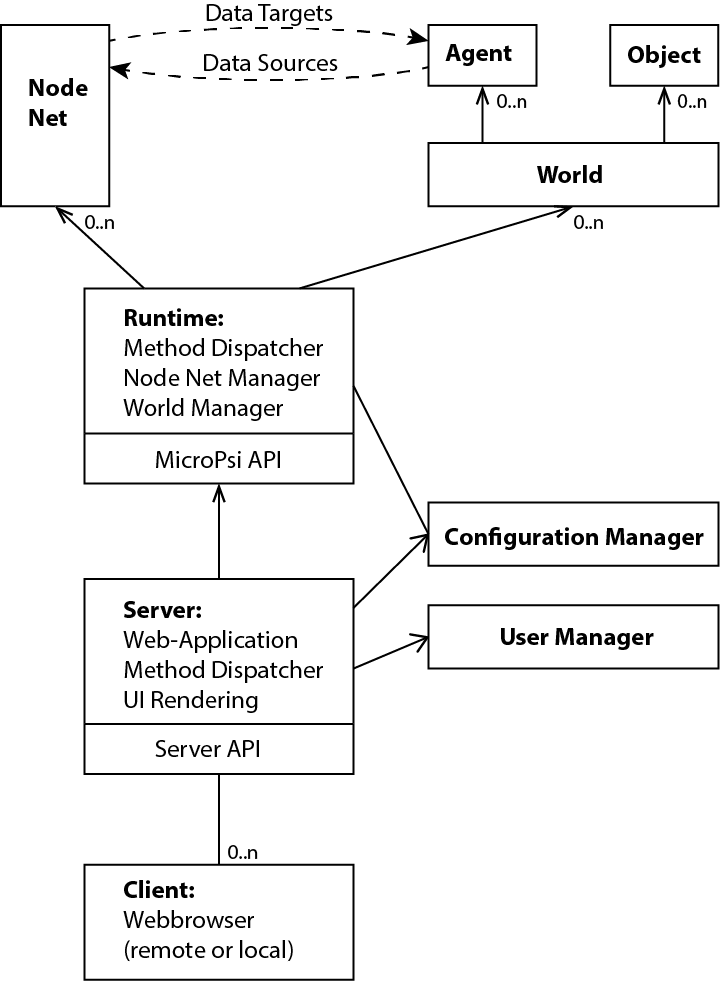
\includegraphics[width=5cm]{graphics/micropsi2_uml}
            
            \paragraph{Agents}
"MicroPsi interprets cognitive models as agents, situated in dynamic environments. MicroPsi agents are entirely defined as hierarchical spreading activation networks (SAN), which—for lack of a better name—are called node nets. Node nets are the brains of these agents—or rather, an abstraction of the information processing provid- ed by brains, and the environment provides a body and stuff to interact with.
The body manifests itself as a set of data sources (which can be thought of as the terminals of sensory neurons) and data targets (the abstracted equivalent of motor neurons). By reading activation values from data sources, and sending activation into data targets, the MicroPsi agent may control its body and interact with its world.
MicroPsi’s node nets can be interpreted as neural networks and afford neural learn- ing paradigms. For the purposes of information storage and retrieval, they can be seen as semantic networks with a small set of typed links to express associative, partonom- ic, taxonomic and causal relationships.
Since the nodes can also encapsulate state machines and arbitrary operations over the node net, they can also be understood as components of a concurrent, modularized architecture, with activation spreading as the primary means of communication be- tween the modules."~\cite{conf/agi/Bach12}

            \paragraph{Environment}
"Within the MicroPsi framework, agents may be embedded into an environment (world). The environment must provide a world adapter wa for each MicroPsi agent. The world adapter offers data sources, from which the agent’s node net may read environmental information, and data targets, which allow the agent to effect changes in the world. Since the environment only has write access to data sources, and read access to data targets, node net and environment may be updated asynchronously.
The world adapter may interface a local multi-agent simulation, a robotic body, a computer game client or simulation server, dynamically updated stock data, etc."~\cite{conf/agi/Bach12}

            \paragraph{Applications}
"Compared with the original implementation of MicroPsi, the current iteration of the framework is still fragmentary; at the time of writing, it supports only a simple generic simulation world for multi agent experiments (instead of the various simula- tion environments provided in MicroPsi 1). Also, 3D viewing components for envi- ronments and facial expressions are completely absent.
The current priority of MicroPsi 2 lies on affective simulation for problem solving experiments (see Bach 2012b), and its application as a general framework for knowledge representation in a hierarchical semantic network."~\cite{conf/agi/Bach12}


        \subsubsection{Core}
... the core runs the heart of the simulation ...

        \subsubsection{Server}
... the server provides the interface ...

        \subsubsection{Simulation Environments}
... so far, there are an "Island" and an "Berlin" worlds ...

    \section{A! Minecraft}
... a more complex simulation environment could be fun ...

... the story of Minecraft ...
... Minecrafts poularity (and demographics) ...

Video games are natural applications of artificial intelligence. The quality of a games A.I. can make all the difference in between a great title and an unenternaining demo of computer graphics.

One computer-game in particular stood out in the last years --- not for A.I. reasons though. It is called Minecraft and is benefiting of high popularity ever since its first release in 2009. Since copies of the game can be obtained commercially for the first time in 2011, the different versions of the game sold more than 26 million times - the PC version priced at about 20 Euros. It should be noted, that the games developer studio Mojang is a so called "Indie" developer that is not associated with any classical game publisher but distributes copies of their game exclusively via their own website.

Even though the game can be downloaded and played as a single packet of software, many scenarios of playing the game consist of running a Minecraft server software as well as one client per player. It is possible to mimic the official client by implementing the reverse-engineered Client-Server-Protocol and build artificial players that way.

Minecraft is a complex yet easily accesible virtual world. It is constantly developed and new features are added regularly. It is a massive fanbase and a huge community of gamemodifications.

Another interesting aspect about Minecraft is the procedural semantic the game world is generated with and. Trees in Minecraft, for example, may share a similar structure that consists of a trunk and branches and leaves spreading out as fractals, but the particular charecteristics of each tree are generated randomly. This makes a Minecraft world somewhat more realistic than most other videogames.

        \subsection{What is Minecraft?}
... brief description of the basic mechanisms ...

        \subsection{The Cient Server Protokoll}
... the language an external client needs to speak, to take place in a Minecraft world ...

        \subsection{Suitability of Minecraft as a simulation environment}
... cheap licenses ...
... developer friendly community and game-studio ...
... sandbox game with many possibilieties but no pre-defined goals ...
... procedural semantic ...

    \section{A! Minecraft and MicroPsi}
... a more complex simulation environment could be fun ...